\documentclass[../main.tex]{subfiles}

\begin{document}
In questa sezione si analizzano alcune delle librerie scelte per la sperimentazione del paradigma FRP in Scala. Aspetti cruciali dell'analisi delle librerie sono la correttezza rispetto la definizione del paradigma FRP (discussa nel capitolo 2), lo stato attuale della libreria (active, maintenance o EOL) ed il supporto a Scala. La sperimentazione è stata effettuata sviluppando gli stessi esempi con le diverse librerie in analisi: \textit{Sodium}, \textit{Reactify}. Gli esempi sviluppati sono i seguenti:
\begin{itemize}
    \item Sensore di temperatura (\textit{XThermalManagerExample}): flusso di rilevamenti simulati di sensori di temperatura e lavorazioni sui valori per estrarre altri valori come temperatura media e spikes.
    \begin{figure}[H]
        \centering
        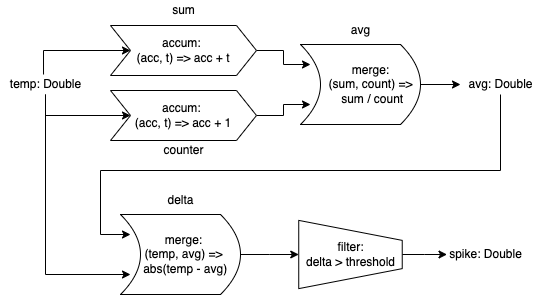
\includegraphics[width=0.9\textwidth]{img/frp-scala-Page-3.drawio.png}
        \caption{Parte del grafo delle dipendenze: temperatura media e spikes}
    \end{figure}
    \item Contatore/ticker (\textit{XTimeFlowExample}): flusso di cambiamenti al valore del contatore, al quale è associata come reazione il calcolo dei millisecondi trascorsi e la stampa del valore.
    \begin{figure}[H]
        \centering
        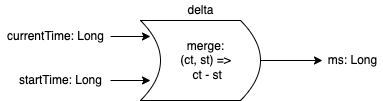
\includegraphics[width=0.7\textwidth]{img/frp-scala-Page-4.drawio.png}
        \caption{Grafo delle dipendenze: timer}
    \end{figure}
\end{itemize}

\section{Sodium}
La libreria open-source Sodium è stata progettata e sviluppata da Stephen Blackheath e Anthony Jones (più altri collaboratori) per fornire una libreria production-ready in diversi linguaggi, tra cui Scala, per promuovere la vera definizione del paradigma FRP e per realizzare un riferimento/benchmark per future librerie.

\begin{table}[H]
\centering
\begin{tabular}{|c|c|}
     \hline
     Repository & https://github.com/SodiumFRP/sodium \\
     \hline
     Versione Latest Release & 1.2.0 \\
     \hline
     Data Latest Release & Ottobre 2019 \\
     \hline
     Data Latest Commit & 3 Febbraio 2020 \\
     \hline
     Supporto Scala & 2.12 \\
     \hline
     Dipendenza Gradle & nz.sodium:sodium:1.2.0 \\
     \hline
\end{tabular}
\caption{Main Info Libreria Sodium}
\end{table}

Nonostante la libreria sia distribuita tramite il repository Maven Central (\url{https://mvnrepository.com/artifact/nz.sodium/sodium/1.2.0}) è stato necessario un fork, disponibile al repo \url{https://github.com/paganellif/sodium} per i seguenti motivi:
\begin{enumerate}
    \item Il package jar della libreria disponibile su maven central è ottenuto dalla pacchettizzazione del sorgente Java. Seppur ci sia grande interoperabilità tra Scala e Java non è possibile sfruttare direttamente le features del linguaggio funzionale. 
    \item Creato il jar partendo dal sorgente Scala sono stati risolti errori/warning permettendo alla libreria di supportare anche Scala 2.13.7, versione utilizzata nel progetto.
\end{enumerate}

\subsection{SodiumThermalManagerExample}
L'entità \textit{SodiumTempSensor} modella un sensore di temperatura che, dato in input un range di valori decimali e la frequenza di spike, ovvero la probabilità che una rilevazione della temperatura da parte del sensore sia sbagliata, emette uno stream di valori decimali rappresentanti la temperatura misurata.

\begin{figure}[H]
    \centering
    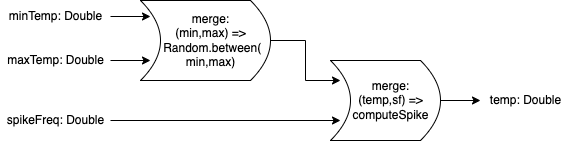
\includegraphics[width=0.9\textwidth]{img/frp-scala-Page-7.drawio.png}
    \caption{Grafo delle dipendenze: TempSensor}
\end{figure}

Lo stream di output del sensore di temperatura, modellato con il costrutto della libreria \textit{Stream[Double]}, rappresenta quindi l'input del componente \textit{SodiumThermalManager}. 

\begin{lstlisting}[language=Javascript, caption=Sodium - Traduzione della parte di grafo delle dipendenze riguardante la temperatura media e gli spike in codice]
implicit class StreamCounter[A](stream: Stream[A]) {
  def count(): Stream[Int] = stream
    .accum(0, (t: A, acc: Int) => acc + 1).updates()
}
  
def sumTemp: Stream[Double] = tempSensor.temp
  .accum(0.0, (t: Double,acc: Double) => acc + t).updates()
    
def firingCount: Stream[Int] = tempSensor.temp.count()

def avgTemp: Stream[Double] = sumTemp.merge(firingCount.map(i => i.toDouble), (s,f) => s / f)

def spikeTemp: Stream[Double] = tempSensor.temp
  .merge(avgTemp, (t, avg) => Math.abs(t - avg)).filter(t => t > thresholdTemp.sample())
\end{lstlisting}

La traduzione in codice del grafo delle dipendenze progettato è possibile grazie alle primitive fornite dalla libreria Sodium, la quale ne aggiunge altre a quelle basiche viste nel capitolo precedente. Un esempio di primitiva aggiuntiva e utilizzata per computare la somma delle temperatura è la primitiva \textit{accum}.

Dato l'output del \textit{SodiumThermalManager} viene registrato come handler una semplice stampa a console di test del valore:
\begin{lstlisting}[language=Javascript, caption=Sodium - Registrazione listeners]
avgTemp.listen(avg => println(s" avg: $avg"))
spikeTemp.listen(spike => println(s"spike: $spike"))
\end{lstlisting}

\subsection{SodiumTimeFlowExample}
Un esempio di test più banale rispetto a quello precedente è la realizzazione di un contatore/ticker: dato il tempo iniziale in millisecondi modifica il valore di una variabile con una certa cadenza periodica, emettendo quindi un flusso di cambiamenti.

\begin{lstlisting}[language=Javascript, caption=Sodium - Esempio completo]
val startTime: Cell[Long] = new Cell(System.currentTimeMillis())
val currentTime: StreamSink[Long] = new StreamSink[Long]()

currentTime.map(ct => ct - startTime.sample())
  .listen(ms => println(s"ms: $ms"))

new Thread(() => {
  while(true) {
    currentTime.send(System.currentTimeMillis())
    sleep(500)
  }
}).start()
\end{lstlisting}

\section{Reactify}
Reactify è una libreria open-source che permette di sviluppare sistemi col paradigma FRP fornendo un insieme limitato di concetti rispetto ad altre librerie come Sodium. Il programma viene espresso in termini di variabili che cambiano (\textit{Var}) o non cambiano (\textit{Val}) valore nel tempo e nel definire una reazione al cambiamento: tutte le primitive tipiche del paradigma FRP non sono fornite dalla libreria, la quale permette di usare qualsiasi funzionalità di Scala direttamente.

\begin{table}[H]
\centering
\begin{tabular}{|c|c|}
     \hline
     Repository & https://github.com/outr/reactify \\
     \hline
     Versione Latest Release & 4.0.6 \\
     \hline
     Data Latest Release & Maggio 2021 \\
     \hline
     Data Latest Commit & 17 Maggio 2021 \\
     \hline
     Supporto Scala & 2.11, 2.12, 2.13, 3 \\
     \hline
     Dipendenza Gradle & com.outr:reactify\_2.13:4.0.6 \\
     \hline
\end{tabular}
\caption{Main Info Libreria Reactify}
\end{table}

\subsection{ReactifyThermalManagerExample}
% a differenza di sodium esistono solo var ( == Cell) e val ( == Stream)
% le dipendenze del grafo sono definite da quello che si inserisce dentro alle val:
% per definire le dipendenze è possibile usare qualsiasi costrutto fornito da scala (a differenza di sodium che fonirsce le primitive) basandosi su delle var reactify
% cioè, quando una var cambia valore allora ogni val che contiene il suo riferimento viene ricalcolata in reazione al cambiamento ma NON ESISTONO PRIMITIVE 

\subsection{ReactifyTimeFlowExample}

\end{document}

